\setcounter{figure}{0}
\setcounter{lstlisting}{0}
\section{Vježba 6: Određivanje dominantne ravnine na 2.5D slici RANSAC
metodom}

\subsection{Opis vježbe}
Omogućiti korisniku učitavanja 2.5D slike, prethodno snimljene Kinect
kamerom. Učitanu sliku potrebno je prikazati kao crno bijelu sliku na
način da se dubina predstavi kao intenzitet crne boje. Na slici je
potrebno pronaći dominantu ravninu te ju označiti bojom.
\\

\subsection{Objašnjenje programa}
Ovaj program se nakon učitavanja slika s Kineckt kamere svodi na RANSAC
algoritam i dvije funkcije. Prva funkcija je \textit{isPlane()} koja
provjera jesu li odabrane točke na istoj ravnini (dubini). Te druge
funkcije \textit{planePoints()} koja prebrojava sve točke pronađene
ravnine.
\subsubsection{Dominantna ravnina}
\begin{lstlisting}[language=C,caption={Dominant plane}]
int main (int argc, char *argv[])
{
    /* Code for image loading */
    // Use RANSAC to determine dominant plane
    srand(time(NULL));
    int ransacRounds = 1000;
    int bestPlane = 0;
    for (int i = 0; i < ransacRounds; i++) {
        vector<float> points, depth, plane;
        points.clear(); depth.clear(); plane.clear();
        // Choose 3 random points and their depth
        for (int j = 0; j < 3; j++) {
            int u = rand (0, img.cols);
            int v = rand (0, img.cols);
            int d = imgDepth.at<uchar>(v,u);
            points.push_back((float)u);
            points.push_back((float)v);
            points.push_back(1.0f);
            depth.push_back((float)d);
        }
        // Check if points are on the same plane else skip iteration
        if (!isPlane (points, depth, &plane))
            continue; 
        // Calculate number of points on the same plane
        int num = planePoints (&imgDepth, plane);
        if (num > bestPlane) {
            bestPlane = num;
            bPlane.swap(plane);
        }
    }
    /* Code for marking and showing result */
    return 0;
}
bool isPlane (vector<float> points, vector<float> depth, vector<float> *plane) 
{
    Mat A_(3, 3, CV_32FC1, &points[0]);
    Mat Z_(3, 1, CV_32FC1, &depth[0]);
    Mat p_(3, 1, CV_32FC1);
    // Solves linear system with three equations
    // if there is solution save plane location
    if (solve(A_, Z_, p_)) {
        for (int i = 0; i < 3; i++) plane->push_back(p_.at<float>(i));
        return 1; // valid points
    } else
        return 0; // selected points are on the same line
}
int planePoints (Mat *depth, vector<float> plane) 
{
    float thr = 4.0f; // threshold
    int nMatch = 0; // number of matches
    // Calculate number of points on the sam plain
    for (int j = 0; j < depth->rows; j++) {
        for (int i = 0; i < depth->cols; i++) {
            uchar d = depth->at<uchar>(j,i);
            float err = (float)d - (plane[0] * i + plane[1] * j + plane[2]);
            if (err < 0) err *= -1;
            if (err > thr)
                continue;
            else
                nMatch++;
        } }
    return nMatch;
}
\end{lstlisting}

\begin{figure}
\centering
\begin{minipage}{.5\textwidth}
  \centering
  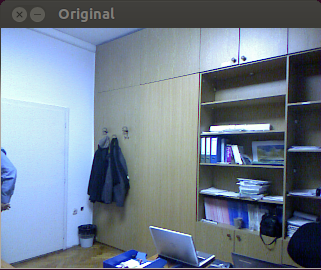
\includegraphics[width=.9\linewidth]{images/lab6-sample-01-or.png}
  \caption{sample-01-original}
  \label{fig:sample-01-original}
\end{minipage}%
\begin{minipage}{.5\textwidth}
  \centering
  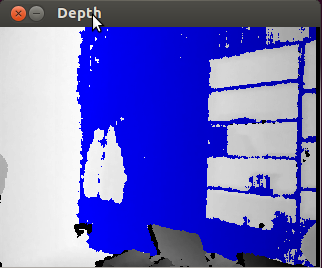
\includegraphics[width=.9\linewidth]{images/lab6-sample-01-dp.png}
  \caption{sample-01-depth}
  \label{fig:sample-01-depth}
\end{minipage}
\end{figure}

\begin{figure}
\centering
\begin{minipage}{.5\textwidth}
  \centering
  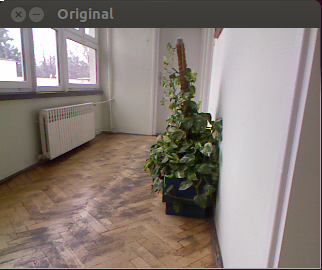
\includegraphics[width=.9\linewidth]{images/lab6-sample-02-or.png}
  \caption{sample-02-original}
  \label{fig:sample-02-original}
\end{minipage}%
\begin{minipage}{.5\textwidth}
  \centering
  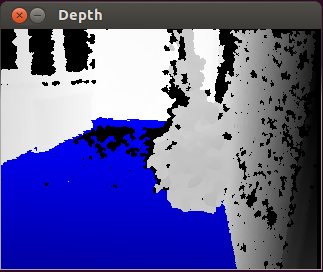
\includegraphics[width=.9\linewidth]{images/lab6-sample-02-dp.png}
  \caption{sample-02-depth}
  \label{fig:sample-02-depth}
\end{minipage}
\end{figure}

\begin{figure}
\centering
\begin{minipage}{.5\textwidth}
  \centering
  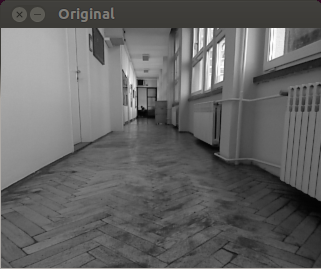
\includegraphics[width=.9\linewidth]{images/lab6-sample-03-or.png}
  \caption{sample-03-original}
  \label{fig:sample-03-original}
\end{minipage}%
\begin{minipage}{.5\textwidth}
  \centering
  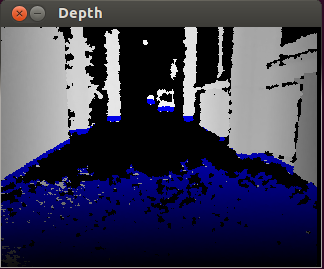
\includegraphics[width=.9\linewidth]{images/lab6-sample-03-dp.png}
  \caption{sample-03-depth}
  \label{fig:sample-03-depth}
\end{minipage}
\end{figure}

\subsection{Zaključak}
Cilj ove vježbe bio je odrediti dominantnu ravninu. Dominantna je
ravnina ploha koja sadrži najviše točaka. Određuje se računanjem
jednadžbi ravnina i prebrojavanjem njihovih pripadajućih točaka. 
Budući da je
algoritam određivanja jednadžbi ravnina pozivan iz RANSAC algoritma
bilo je potrebno postaviti dovoljno velik broj iteracija kako bi
algoritam pronašao sve ravnine i njihove točke. Eksperimentom smo
utvrdili da je 1000 iteracija dovoljno. 

